\documentclass[letterpaper,10pt,conference]{ieeeconf}
\IEEEoverridecommandlockouts
\usepackage{amsmath,amssymb}
\let\proof\relax
\let\endproof\relax
\usepackage{amsthm}
\usepackage{graphicx,booktabs,cite}
\usepackage[hidelinks]{hyperref}
\hypersetup{pdftitle={Deciding Without Waiting: Delay Thresholds for Decentralized Decisions},pdfauthor={Scott Moeller and Bhaskar Krishnamachari},pdfsubject={IEEE Control Systems Letters manuscript},pdfkeywords={Decentralized control, Sensor fusion, Control system architecture}}
\newtheorem{lemma}{Lemma}
\newtheorem{theorem}{Theorem}
\newtheorem{proposition}{Proposition}
\newtheorem{corollary}{Corollary}
\newcommand{\E}{\mathbb E}
\newcommand{\Var}{\operatorname{Var}}
\newcommand{\Cov}{\operatorname{Cov}}
\title{Deciding Without Waiting:\\Delay Thresholds for Decentralized Decisions}
\author{Scott Moeller and Bhaskar Krishnamachari%
\thanks{S. Moeller is an independent researcher, Portsmouth, RI, USA
(\texttt{scott.h.moeller@gmail.com}).}%
\thanks{B. Krishnamachari is with the University of Southern California,
Los Angeles, CA, USA (\texttt{bkrishna@usc.edu}), and is the corresponding author.}}
\begin{document}
\maketitle
\thispagestyle{empty}
\pagestyle{empty}
\begin{abstract}
Fresh local measurements can yield better team decisions than a delayed pool containing every sensor's data. We derive the exact delay threshold in a Gaussian team that tracks a changing signal and penalizes disagreement among agents. The signal and sensor errors share a temporal decay rate. When agents retain fresh local observations, a single pooled scalar achieves the optimal performance of full delayed sharing. Its coordination value decays at twice the signal's correlation decay rate, so the value half-life is half the signal's correlation half-life. We derive the optimal policies, posterior variances, and the value of retaining one local sample from the pooling time. The pooling law extends to unequal sensor quality and independent components with different temporal rates. With a cost per pooled update, an explicit communication-price threshold, or equivalent latency threshold, determines when no refreshing is optimal. Below this threshold, the optimal periodic interval is unique, and periodic refreshing is optimal among all schedules independent of the sensor processes.
\end{abstract}
\noindent\textbf{Index Terms---}Decentralized control, sensor fusion, control system architecture.

\section{Introduction}
Sharing every sensor's data can lead to worse team decisions than acting locally. Collecting and distributing the data takes time, and a changing environment can make a broad view outdated before it is used. We identify the exact delay beyond which fresh local measurements outperform a complete delayed observation pool. Both decision rules are optimized for their available information. In an eight-sensor example, local operation has about $26\%$ lower team loss than decisions based on a pool one coherence time ($1/\lambda$) old, before any communication charge is included.

We consider agents tracking a common changing signal through noisy local sensors. Their shared objective penalizes tracking error and disagreement among their actions. The signal and sensor errors evolve as Gaussian processes with a common temporal decay rate $\lambda$. Agents can use fresh local information, a delayed pool, or a hybrid of both. Actions do not affect future observations, so each decision is a static team problem.

The main results are:
\begin{enumerate}
\item \emph{Optimal decisions and a delay threshold.} We derive fresh-local and fresh-pooled policies, posterior variances, and costs, then identify exactly when local decisions outperform a delayed pool (Proposition~\ref{prop:endpoints}, Corollary~\ref{cor:crossover}).
\item \emph{Hybrid pooling and local memory.} We derive the optimal hybrid policy, its posterior variance, and its exponentially decaying coordination value. We also quantify the loss from discarding the local sample taken at the pooling time (Theorem~\ref{thm:hybrid}, Proposition~\ref{prop:current}).
\item \emph{Unequal quality and temporal rates.} We extend the law to unequal sensor variances and to independent components with different rates (Proposition~\ref{prop:hetero}, Corollary~\ref{cor:modes}).
\item \emph{When and how often to refresh.} We derive price and latency thresholds for choosing no refreshes and prove periodic optimality among all schedules independent of the observations (Theorem~\ref{thm:refresh}).
\end{enumerate}
Static team theory gives optimality conditions for agents with different observations \cite{radner1962team}, and common-information methods separate shared and private information \cite{afshari2017static}. The hybrid is a compressed delayed-sharing architecture, following the information pattern introduced by Witsenhausen \cite{witsenhausen1971separation} and studied by Nayyar, Mahajan, and Teneketzis \cite{nayyar2011sharing}. Theorem~\ref{thm:hybrid} shows that a single scalar broadcast achieves the value of full delayed sensor sharing in this model.

Age of information \cite{yates2021aoi}, nonlinear age penalties \cite{sun2017update}, and remote estimation \cite{ornee2021ou} connect freshness to performance. Ballotta and coauthors show that communication latency can make sparse consensus controllers outperform centralized control \cite{ballotta2023latency}, and study optimal feedback locality in spatially invariant systems \cite{ballotta2026role}. Here, a static team driven by an Ornstein--Uhlenbeck signal yields a closed-form delay crossover, an exact hybrid pooling law, and optimal refresh scheduling.

Kar and Varshney study sensor collaboration and sampling of an Ornstein--Uhlenbeck signal under a power budget \cite{kar2012controlled}. Nayyar, Ba\c{s}ar, Teneketzis, and Veeravalli jointly optimize communication and remote estimation under communication costs and energy constraints \cite{nayyar2013optimal}. Their transmission decisions can depend on sensor observations. Our setting gives every agent fresh private observations between pooled updates and penalizes disagreement among decisions. The exact age law quantifies the value of the shared update in this team, and the refresh theorem optimizes schedules chosen independently of observed values.

A longer version of this paper \cite{tina2026} develops a broader theory of information architecture, covering local versus delayed-global information, spatial predictability, and neighborhood-radius selection. This letter gives a self-contained analysis of common-signal Gaussian teams, including all proofs of the pooling and refresh results.

\section{The Team and Its Information}
\subsection{Signal, observations, and objective}
There are $n\ge2$ agents with scalar actions $u_i(t)$. The common signal $X(t)$ and sensor disturbances $E_i(t)$ are mutually independent, zero-mean, stationary Gaussian processes with
\begin{align}
 \Cov(X(t),X(s))&=a e^{-\lambda|t-s|},\notag\\
 \Cov(E_i(t),E_i(s))&=b e^{-\lambda|t-s|},\label{eq:model}
\end{align}
where $a,b,\lambda>0$. Each is an Ornstein--Uhlenbeck process \cite{uhlenbeck1930brownian}. Agent $i$ observes
\begin{equation}
 Y_i(t)=X(t)+E_i(t),\qquad \bar Y(t)=\frac1n\sum_iY_i(t).
 \label{eq:observations}
\end{equation}
The disturbance represents temporally correlated local measurement error. The coherence time $1/\lambda$ is the lag at which correlation falls to $e^{-1}$. The common rate in \eqref{eq:model} makes all temporal covariances share one factor. Consequently, the instantaneous pooled residual $\eta$ in \eqref{eq:eta} is independent of the entire sensor history, and current readings suffice for the endpoint policies. With independent measurement noise at successive sample times, the local posterior generally requires a Kalman filter that incorporates past readings. The single-reading reduction then fails.

At each time the team minimizes the expected loss
\begin{equation}
 \ell(u,X)=\frac1n\sum_i(u_i-X)^2
       +\frac\kappa n\sum_i(u_i-\bar u)^2,
 \quad \bar u=\frac1n\sum_i u_i,\label{eq:loss}
\end{equation}
where $\kappa\ge0$. The terms price tracking error and disagreement. Actions affect neither the processes nor the observations. The problem is a sequence of static team decisions. All measurable policies with finite second moment are admissible when they satisfy the stated information restrictions.

\subsection{Architectures and stored information}
Write $\mathcal F_i(t)=\sigma\{Y_i(r):r\le t\}$ for the local history and $\mathcal F(t)=\bigvee_i\mathcal F_i(t)$ for the full sensor history. Fresh-local operation gives agent $i$ the information $\mathcal F_i(t)$. Fresh-pooled operation gives every agent $\mathcal F(t)$. At pooling time $s=t-\tau$, delayed-pool-only operation gives every agent $\mathcal F(s)$ and uses no measurements taken after $s$. The hybrid architecture retains the local history through $t$ and has information
\begin{equation}
 \mathcal H_i(t;s)=\mathcal F_i(t)\vee
             \sigma\{\bar Y(r):r\le s\}.\label{eq:hybrid}
\end{equation}
Its pool is $\tau$ time units old and its local information is current. Let $J_L$, $J_P$, $J_D(\tau)$, and $J_H(\tau)$ be the respective minimum expected losses. Table~\ref{tab:information} lists the data sufficient for the optimal policies. Section~III proves that the hybrid value is unchanged when pooled information arrives only at selected refresh times.

We call $J_L-J_H(\tau)$ the \emph{coordination value} of the delayed pool. It includes reductions in tracking error and disagreement. Its age-zero value is $\Delta=J_L-J_P$.

\begin{table}[t]
\caption{Data sufficient to implement the optimal policies. The last row restricts each device to its current local reading.}
\label{tab:information}
\centering
\begin{tabular}{@{}lll@{}}
\toprule
Architecture & Local data used & Shared scalar \\
\midrule
Fresh-local & $Y_i(t)$ & None \\
Fresh-pooled & None & $\bar Y(t)$ \\
Delayed pool only & None & $\bar Y(s)$ \\
Hybrid & $Y_i(t),Y_i(s)$ & $\bar Y(s)$ \\
Current reading + pool & $Y_i(t)$ & $\bar Y(s)$ \\
\bottomrule
\end{tabular}
\end{table}

\subsection{Optimality and the fresh endpoints}
The following specialization of Radner's stationarity condition \cite{radner1962team} applies to all admissible policies.
\begin{lemma}[Team optimality]\label{lem:normal}
For information fields $\mathcal G_i$, a feasible policy $u$ is optimal if and only if
\begin{equation}
 (1+\kappa)u_i-\kappa\E[\bar u\mid\mathcal G_i]
       =\E[X\mid\mathcal G_i],\qquad i=1,\ldots,n.\label{eq:normal}
\end{equation}
The optimal policy is unique up to almost-sure equality.
\end{lemma}
\begin{proof}
For feasible $w$, the first variation is $2n^{-1}\sum_i\E[w_i((1+\kappa)u_i-\kappa\bar u-X)]$ and vanishes for all $w$ exactly when \eqref{eq:normal} holds. The remainder is $n^{-1}\sum_i\E[w_i^2+\kappa(w_i-\bar w)^2]>0$ for $w\ne0$, proving necessity, sufficiency, and uniqueness.
\end{proof}
Define
\begin{equation}
 v=a+\frac bn,\qquad d=a+b\left[1+\kappa\left(1-\frac1n\right)\right].\label{eq:vd}
\end{equation}
\begin{proposition}[Fresh endpoints]\label{prop:endpoints}
The posterior variances are
\begin{align}
 P_1=\Var(X(t)\mid\mathcal F_i(t))&=\frac{ab}{a+b},\notag\\
 P_n=\Var(X(t)\mid\mathcal F(t))&=\frac{ab}{b+na}.\label{eq:posterior}
\end{align}
The optimal policies and costs are
\begin{align}
 u_i^L(t)&=\frac ad Y_i(t),& J_L&=a-\frac{a^2}{d},\label{eq:local}\\
 u_i^P(t)&=\frac av\bar Y(t),& J_P&=P_n=a-\frac{a^2}{v}.\label{eq:pooled}
\end{align}
In particular,
\begin{equation}
 \Delta=\frac{a^2(d-v)}{vd}>0.\label{eq:delta}
\end{equation}
\end{proposition}
\begin{proof}
For any $r\le t$, the residual $X(t)-aY_i(t)/(a+b)$ has zero covariance with $Y_i(r)$. Gaussianity makes it independent of the local history. Similarly,
\begin{equation}
 \eta(t)=X(t)-\frac av\bar Y(t)\label{eq:eta}
\end{equation}
has zero covariance with $Y_j(r)$ for every $j$ and every $r$. It is independent of the full sensor process. Computing the residual variances gives \eqref{eq:posterior} and the corresponding conditional means.

For $u_i=kY_i(t)$,
$\E[\bar u\mid\mathcal F_i(t)]=kvY_i(t)/(a+b)$.
Equation~\eqref{eq:normal} then gives
$k[(1+\kappa)(a+b)-\kappa v]=a$.
The bracket equals $d$, proving the local policy. Its expected loss is $a-2ak+dk^2=a-a^2/d$. With pooled information, every agent uses the same conditional mean of $X(t)$, with zero disagreement and loss $P_n$. Lemma~\ref{lem:normal} proves optimality. Finally, $d-v=b(1+\kappa)(1-1/n)>0$ gives \eqref{eq:delta}.
\end{proof}
When $\kappa>0$, the local action has smaller magnitude than the local posterior mean. The team trades some individual tracking accuracy for less disagreement. Specifically,
\begin{equation}
 J_L-P_1=\frac{\kappa a^2b(1-1/n)}{(a+b)d}.\label{eq:localgap}
\end{equation}
Pooling removes this additional cost and reduces posterior variance.

\section{An Exact Law for Delayed Pooling}
\subsection{When local decisions outperform pooling}
Pooling provides a common estimate from all sensors. Its age determines whether that estimate supports better decisions than current local measurements.
\begin{corollary}[The delay crossover]\label{cor:crossover}
Under delayed-pool-only information, the optimal policy and loss are
\begin{equation}
 u_i^D(t)=e^{-\lambda\tau}\frac av\bar Y(s),\qquad
 J_D(\tau)=a-\frac{a^2}{v}e^{-2\lambda\tau}.\label{eq:delayedonly}
\end{equation}
Fresh-local operation has strictly smaller team loss precisely when
\begin{equation}
 \tau>\tau_{\rm cross}:=\frac{1}{2\lambda}\log\frac{d}{v}.\label{eq:crossover}
\end{equation}
The two costs agree at $\tau=\tau_{\rm cross}$.
\end{corollary}
\begin{proof}
The Markov property and Proposition~\ref{prop:endpoints} give
$\E[X(t)\mid\mathcal F(s)]=e^{-\lambda\tau}(a/v)\bar Y(s)$. Taking this common conditional mean minimizes tracking loss and gives zero disagreement, hence also minimizes the team loss. Its error variance is \eqref{eq:delayedonly}. Comparing with $J_L=a-a^2/d$ gives $J_L<J_D$ exactly when $e^{-2\lambda\tau}<v/d$, which is \eqref{eq:crossover}.
\end{proof}
This crossover compares decision losses alone. Stronger disagreement penalties increase $d$ and therefore increase the delay that pooling can tolerate. Faster temporal change increases $\lambda$ and shortens that tolerance.

\subsection{Retaining fresh local information}
The hybrid keeps current local measurements available while the pool ages. The next theorem gives its exact improvement over local operation.
\begin{theorem}[Hybrid policy and exponential value]\label{thm:hybrid}
Let $s=t-\tau$ and $\rho=e^{-\lambda\tau}$. Under \eqref{eq:model}--\eqref{eq:hybrid}, the optimal hybrid policy is
\begin{equation}
 u_i^H(t)=\rho\frac av\bar Y(s)
       +\frac ad\bigl(Y_i(t)-\rho Y_i(s)\bigr).\label{eq:hybridpolicy}
\end{equation}
It attains the optimum even if every agent receives all sensor histories through $s$. The posterior variance $P_H(\tau)=\Var(X(t)\mid\mathcal H_i(t;s))$ and team cost satisfy
\begin{align}
 P_H(\tau)&=\rho^2P_n+(1-\rho^2)P_1,\label{eq:phybrid}\\
 J_H(\tau)&=\rho^2J_P+(1-\rho^2)J_L.\label{eq:jhybrid}
\end{align}
Consequently,
\begin{equation}
 J_L-J_H(\tau)=\Delta e^{-2\lambda\tau}.\label{eq:exponential}
\end{equation}
\end{theorem}
\begin{proof}
For $\tau=0$, \eqref{eq:hybridpolicy} is the pooled policy. Suppose $\tau>0$ and enlarge each agent's information to $\mathcal G_i=\mathcal F(s)\vee\mathcal F_i(t)$. Set
\begin{equation}
 Z_i=Y_i(t)-\rho Y_i(s),\quad h=\frac av,\quad k=\frac ad.\label{eq:innov}
\end{equation}
The Gaussian Markov property makes $Z=(Z_1,\ldots,Z_n)$ independent of $\mathcal F(s)$, with covariance $(1-\rho^2)(a\mathbf1\mathbf1^\top+bI)$. Equation~\eqref{eq:eta} gives
\begin{equation}
 X(t)=\rho h\bar Y(s)+h\bar Z+\eta(t).\label{eq:targetdecomp}
\end{equation}
The last term is independent of all sensor data and has variance $P_n$.

For $s<r\le t$, let $Z_i(r)=Y_i(r)-e^{-\lambda(r-s)}Y_i(s)$. Directly from \eqref{eq:model},
\begin{equation}
 \Cov(\bar Z,Z_i(r))=\frac{v}{a+b}\Cov(Z_i,Z_i(r)).\label{eq:pathcov}
\end{equation}
Both covariances share the temporal factor $e^{-\lambda(t-r)}(1-e^{-2\lambda(r-s)})$. Thus $\bar Z-vZ_i/(a+b)$ is orthogonal to the entire local innovation path and to $\mathcal F(s)$. Gaussianity gives $\E[\bar Z\mid\mathcal G_i]=vZ_i/(a+b)$. Since $\eta(t)$ is independent of all sensor data,
\begin{align*}
 \E[h\bar Z+\eta(t)\mid\mathcal G_i]&=\frac{a}{a+b}Z_i,\\
 \E[k\bar Z\mid\mathcal G_i]&=\frac{kv}{a+b}Z_i.
\end{align*}
Subtract the common prediction $\rho h\bar Y(s)$ from all actions. Since $(1+\kappa)(a+b)-\kappa v=d$, the correction $kZ_i$ satisfies \eqref{eq:normal} under the full path information $\mathcal G_i$. Lemma~\ref{lem:normal} certifies optimality. The policy \eqref{eq:hybridpolicy} is feasible under \eqref{eq:hybrid}, so it attains the same value as complete delayed sharing.

At one time, $X=h\bar Y+\eta$ separates the local cost into the irreducible term $P_n$ and the remaining cost $J_L-P_n$. Replacing $Y$ by $Z$ scales the latter quadratic cost by $1-\rho^2$. Thus $J_H=P_n+(1-\rho^2)(J_L-P_n)$, giving \eqref{eq:jhybrid}. The posterior mean under the enlarged information is $\rho h\bar Y(s)+aZ_i/(a+b)$. It is feasible under \eqref{eq:hybrid} and has error variance $P_n+(1-\rho^2)(P_1-P_n)$. This proves \eqref{eq:phybrid}. Equation~\eqref{eq:exponential} follows by subtraction.
\end{proof}
Retaining at least a fraction $\alpha\in(0,1)$ of the fresh-pooling value requires
\begin{equation}
 \tau\le\frac{\log(1/\alpha)}{2\lambda}.\label{eq:agebudget}
\end{equation}
This age budget is independent of $n$, $a$, $b$, and $\kappa$. Those parameters determine the amount $\Delta$ of value available to preserve. The value half-life $\log 2/(2\lambda)$ is half the signal's correlation half-life.

The endpoint and pooling results also hold for independent stationary Gaussian AR(1) signal and disturbance processes with a common one-step coefficient $q\in(0,1)$. At age $k$ steps, replace $e^{-\lambda\tau}$ by $q^k$ throughout: the covariance factorization and normal equations are unchanged, and the hybrid gain is $\Delta q^{2k}$. The continuous-time refresh integrals in Section~V become sums in discrete time.

\subsection{The value of retaining a local sample}\label{subsec:memory}
The retained sample permits an exact local innovation calculation. To quantify its value, consider a device that uses only its current reading and the last pooled mean. Its information is $\sigma\{Y_i(t),\bar Y(s)\}$, and let its optimal team cost be $J_C(\tau)$.
\begin{proposition}[Current reading and old pool]\label{prop:current}
Put $z=e^{-2\lambda\tau}$. The coordination value of this architecture is
\begin{equation}
 J_L-J_C(\tau)=\Delta\,\frac{z(d-v)}{d-vz}.\label{eq:currentgain}
\end{equation}
For every $0<\tau<\infty$, it is strictly smaller than the retained-sample value $\Delta z$.
\end{proposition}
\begin{proof}
Let $M=\bar Y(s)$, $R_i=Y_i(t)-\sqrt zM$, and $\widetilde X=X(t)-\sqrt z(a/v)M$. Gaussian regression makes $(\widetilde X,R)$ independent of $M$, with
\begin{align*}
 \Cov(\widetilde X,R_i)&=a(1-z),\\
 \Var(R_i)&=a+b-zv,\qquad
 \Cov(R_i,\bar R)=v(1-z).
\end{align*}
Since $d-zv=(d-v)+(1-z)v>0$, conditioning on $M$ and applying Lemma~\ref{lem:normal} gives the unique optimal policy
\begin{equation}
 u_i=\sqrt z\frac avM+\frac{a(1-z)}{d-zv}R_i.\label{eq:currentpolicy}
\end{equation}
Substitution into the conditional quadratic cost yields
\begin{equation}
 J_C=a-\frac{a^2z}{v}-\frac{a^2(1-z)^2}{d-zv}.\label{eq:currentcost}
\end{equation}
Subtracting this expression from $J_L$ and using \eqref{eq:delta} gives \eqref{eq:currentgain}. For $0<z<1$, $(d-v)/(d-vz)<1$, which proves the strict comparison.
\end{proof}
As age increases, the ratio $(d-v)/(d-vz)$ decreases from $1$ to $1-v/d$. Discarding the stored sample therefore forfeits at most the fraction $v/d$ of the hybrid coordination value, about $39.1\%$ in Section~VI's example.

\section{Unequal Sensor Quality and Temporal Rates}
\subsection{Sensors with different disturbance variances}
The scalar pooling law also permits unequal sensor quality. Let $\Var(E_i(t))=b_i>0$, with the common rate $\lambda$ unchanged, and define
\begin{equation}
 C_i=(1+\kappa)a+b_i[1+\kappa(1-1/n)],
 \quad \theta=\frac1n\sum_i C_i^{-1}.\label{eq:heterodefs}
\end{equation}
\begin{proposition}[Unequal sensor quality]\label{prop:hetero}
The fresh-local coefficients, fresh-pooled posterior, and costs are
\begin{align}
 k_i&=\frac{a}{C_i(1-\kappa a\theta)},&
 J_L&=a-\frac{a^2\theta}{1-\kappa a\theta},\notag\\
 P&=\left(a^{-1}+\sum_i b_i^{-1}\right)^{-1},&
 \mu_P(t)&=P\sum_i\frac{Y_i(t)}{b_i},\label{eq:hetero}
\end{align}
with $u_i^L=k_iY_i$ and $J_P=P$. Broadcasting the single scalar $\mu_P(s)$ gives the hybrid optimum
\begin{equation}
 u_i^H(t)=\rho\mu_P(s)+k_i[Y_i(t)-\rho Y_i(s)],\label{eq:heteropolicy}
\end{equation}
and $J_H=\rho^2J_P+(1-\rho^2)J_L$.
\end{proposition}
\begin{proof}
Substitution of $u_i=k_iY_i$ into \eqref{eq:normal} gives $C_i k_i-\kappa a\bar k=a$, where $\bar k=n^{-1}\sum_i k_i$. Averaging $k_i=(a+\kappa a\bar k)/C_i$ solves for $\bar k$ and gives \eqref{eq:hetero}. The denominator is positive because $C_i>(1+\kappa)a$. Lemma~\ref{lem:normal} then certifies optimality. The quadratic term equals $a\bar k$, so $J_L=a-a\bar k$. Gaussian conditioning gives the displayed $P$ and $\mu_P$.

The residual $X(t)-\mu_P(t)$ is independent of the entire sensor process, since all temporal covariances share the same factor. Innovations over $[s,t]$ have covariance $(1-\rho^2)\Sigma$, where $\Sigma=a\mathbf1\mathbf1^\top+\operatorname{diag}(b_i)$. For $\mathcal G_i=\mathcal F(s)\vee\mathcal F_i(t)$, the covariance argument in \eqref{eq:pathcov} gives $\E[Z_j\mid\mathcal G_i]=\Sigma_{ji}Z_i/\Sigma_{ii}$. After subtracting $\rho\mu_P(s)$, the target has conditional mean $aZ_i/(a+b_i)$. The residual normal equations are therefore the fresh-local equations above, so $k_iZ_i$ is optimal. Scaling the remaining quadratic cost by $1-\rho^2$ gives the stated cost law.
\end{proof}

\subsection{Independent components with different rates}
A task may contain components that change on different time scales. Suppose each agent selects $(u_{i1},\ldots,u_{iM})$ and the loss is $\sum_m w_m\ell_m$, with $w_m>0$. Component $m$ follows the model above with parameters $(a_m,b_m,\kappa_m,\lambda_m)$, and the component processes are mutually independent. Within each component, the common signal and its sensor disturbances share the rate $\lambda_m$. The rates may differ across components. Define $J_{L,m}$, $J_{P,m}$, and $\Delta_m$ by Proposition~\ref{prop:endpoints}.
\begin{corollary}[Additive coordination value]\label{cor:modes}
If the pooled mean $\bar Y_m$ for component $m$ has age $\tau_m$, its optimal policy is \eqref{eq:hybridpolicy} with the corresponding parameters. The total coordination value is
\begin{equation}
 J_L^{\rm tot}-J_H^{\rm tot}=\sum_m w_m\Delta_m e^{-2\lambda_m\tau_m},
 \quad J_L^{\rm tot}=\sum_m w_mJ_{L,m}.\label{eq:modes}
\end{equation}
\end{corollary}
\begin{proof}
For component $m$, observations of the other components are independent of its signal and observations. Averaging a policy over those observations preserves the componentwise information constraints. Convexity ensures that this cannot increase its loss. Optimization therefore separates across components. Apply Theorem~\ref{thm:hybrid} to each and sum with weights $w_m$.
\end{proof}
For a common age $\tau$, write the gain in \eqref{eq:modes} as $V(\tau)$. Its logarithmic decay rate is
\begin{equation}
 -\frac{V'(\tau)}{V(\tau)}=
 \frac{\sum_m2\lambda_m w_m\Delta_m e^{-2\lambda_m\tau}}
 {\sum_m w_m\Delta_m e^{-2\lambda_m\tau}}.\label{eq:effective}
\end{equation}
This is a weighted average of the component rates $2\lambda_m$. Slowly changing components account for a larger share of the remaining value as the pool ages.

\section{Optimal Refreshing under a Communication Cost}
A communication service broadcasts the vector of componentwise pooled means $(\bar Y_1,\ldots,\bar Y_M)$, all sampled at the same time, after a fixed latency $\delta\ge0$. It supports the chosen transmission times without queueing. On reception, each pool's age resets to $\delta$. Agents retain local measurements from the associated sampling time in a timestamped buffer. Each vector costs $c>0$ in units of accumulated team loss. Refresh schedules are independent of all signal and disturbance processes and are locally finite, meaning that every bounded time interval contains finitely many transmissions. Deterministic and independent randomized schedules are allowed.

For joint refreshing of all $M$ components, set
\begin{align}
 \gamma_m&=2\lambda_m,\qquad A_m=w_m\Delta_m e^{-\gamma_m\delta},\notag\\
 B(T)&=\sum_m\frac{A_m}{\gamma_m}(1-e^{-\gamma_mT}).\label{eq:refreshdefs}
\end{align}
Here $B(T)$ is the gain accumulated in duration $T$ after a reception. Periodic refreshing with period $T>0$ has average cost
\begin{equation}
 C(T)=J_L^{\rm tot}+\frac{c-B(T)}{T}.\label{eq:periodcost}
\end{equation}
For a general schedule, the objective is the limiting upper average of expected integrated team loss plus $c$ times the number of transmissions. With no refreshes it equals $J_L^{\rm tot}$.

\begin{theorem}[Optimal refresh period]\label{thm:refresh}
Define
\begin{equation}
 c_{\rm crit}=\sum_m\frac{A_m}{\gamma_m}.\label{eq:threshold}
\end{equation}
If $c\ge c_{\rm crit}$, the schedule with no refreshes attains the minimum average cost $J_L^{\rm tot}$. If $0<c<c_{\rm crit}$, periodic refreshing is optimal among all locally finite schedules independent of the sensor processes. Its period is the unique positive solution of
\begin{equation}
 \sum_m\frac{A_m}{\gamma_m}
 [1-(1+\gamma_mT^*)e^{-\gamma_mT^*}]=c.\label{eq:optimalperiod}
\end{equation}
The minimum average cost is
\begin{equation}
 C(T^*)=J_L^{\rm tot}-\sum_m A_m e^{-\gamma_mT^*}.\label{eq:optimalcost}
\end{equation}
\end{theorem}
\begin{proof}
Put $V_\delta(T)=B'(T)=\sum_m A_me^{-\gamma_mT}$. Differentiating \eqref{eq:periodcost} gives
\begin{equation}
 C'(T)=\frac{H(T)-c}{T^2},\quad H(T)=B(T)-TV_\delta(T).\label{eq:derivative}
\end{equation}
Since $H'(T)=-TV_\delta'(T)>0$, $H$ increases strictly from zero to $c_{\rm crit}$. For $0<c<c_{\rm crit}$, $C$ decreases up to the unique root $H(T^*)=c$ and then increases. Also, $C(T)\to\infty$ as $T\downarrow0$ and $C(T)\to J_L^{\rm tot}$ as $T\to\infty$. These facts prove the unique minimizing period and \eqref{eq:optimalperiod}. At the root, $c-B(T^*)=-T^*V_\delta(T^*)$, proving \eqref{eq:optimalcost}. If $c\ge c_{\rm crit}$, then $c-B(T)\ge0$ for every finite $T$.

To compare general schedules, set $g=\min\{0,\inf_{T>0}(c-B(T))/T\}$. Condition on any realization of an independent reception schedule. Each complete reception interval $T_j$ contributes at least $gT_j$ relative to fresh-local operation after assigning one communication cost to it. The last incomplete interval contributes at least $-c_{\rm crit}$, which bounds the gain over its entire lifetime. The initial interval before any reception has zero gain. Because $g\le0$, the expected total cost through time $R$, conditional on the schedule, is at least
\[
 R(J_L^{\rm tot}+g)-c_{\rm crit}.
\]
Charging transmissions at generation preserves this lower bound because the number sent is at least the number received. The bound is uniform over schedule realizations. Take expectation over the schedule, divide by $R$, and then take the limiting upper average as $R\to\infty$. This proves the bound for independent randomized schedules. Periodic operation at $T^*$, or no communication in the other case, attains it.
\end{proof}
For one component, $x=2\lambda T^*$ and $\chi=c/c_{\rm crit}$ reduce the period equation to
\begin{equation}
 1-(1+x)e^{-x}=\chi,\qquad 0<\chi<1.\label{eq:dimensionless}
\end{equation}
The left side increases strictly, so bisection determines the period. As the price approaches its threshold, the interval diverges. For a single component of unit weight, the no-refresh condition has the equivalent latency form
\begin{equation}
 \delta\ge\delta_{\rm stop}:=\max\left\{0,\frac{1}{2\lambda}\log\frac{\Delta}{2\lambda c}\right\}.\label{eq:latencystop}
\end{equation}
This follows by solving $c\ge\Delta e^{-2\lambda\delta}/(2\lambda)$ for $\delta$. At or above this threshold, every finite periodic refresh schedule has larger total cost than local operation. No refreshes also attain the optimum over the full independent-schedule class in Theorem~\ref{thm:refresh}. If the service requires intervals of at least $T_{\min}>0$, the derivative sign in \eqref{eq:derivative} gives the constrained period $\max\{T_{\min},T^*\}$ below the same threshold.

\section{Numerical Illustration}
Consider $n=8$, $a=b=1$, $\kappa=1$, and $\lambda=1$. Then $P_1=0.5$, $J_P=P_n=1/9$, $J_L=15/23$, and $\Delta=112/207\simeq0.5411$. The delay crossover is $\lambda\tau_{\rm cross}\simeq0.4691$. At one coherence time, $\lambda\tau=1$, delayed-pool-only loss is $0.8797$, compared with $0.6522$ locally. Local operation therefore reduces team loss by $25.9\%$, with no communication price included. At age $\tau=0.5$, the hybrid retains $e^{-1}\simeq36.8\%$ of the fresh-pooling value and has loss $0.4531$.
\begin{figure}[t]
 \centering
 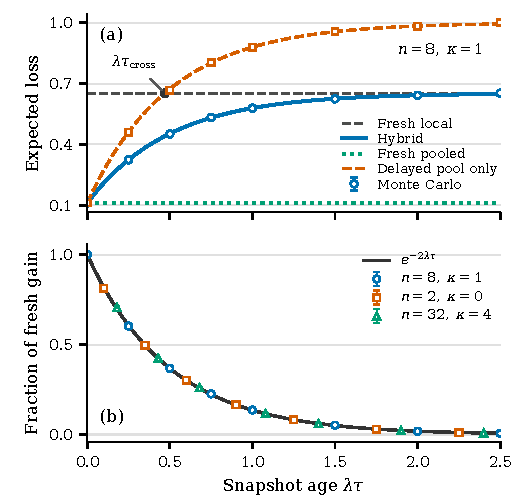
\includegraphics[width=\columnwidth]{figures/pooling_decay.pdf}
 \caption{The delay crossover and hybrid value. A delayed pool used alone becomes worse than fresh-local operation beyond $\tau_{\rm cross}$. The hybrid retains fresh local information and improves on local operation. Its normalized gain follows the exponential law. Markers use stationary Gaussian sample pairs.}
 \label{fig:decay}
\end{figure}
Figure~\ref{fig:decay} uses 120,000 independent stationary Gaussian sample pairs per marker. We also solve the Gaussian team normal equations directly from observation covariances. Across 40 random parameter sets with $2\le n\le12$, $0.1\le a,b\le10$, $0.01\le\kappa\le10^{1.5}$, and $0.01\le\rho\le0.98$, three architectures give 120 systems. Six additional $\kappa=0$ cases check boundary ages. The maximum cost discrepancy across all 126 systems is $5.3\times10^{-15}$.

For latency $\delta=0.1$, the critical communication cost is $\Delta e^{-0.2}/2\simeq0.2215$. Figure~\ref{fig:refresh} shows the effect of communication price. At half this cost, \eqref{eq:dimensionless} gives $2\lambda T^*\simeq1.6783$, hence $T^*\simeq0.8392$. The average cost is approximately $0.5695$. 
\begin{figure}[t]
 \centering
 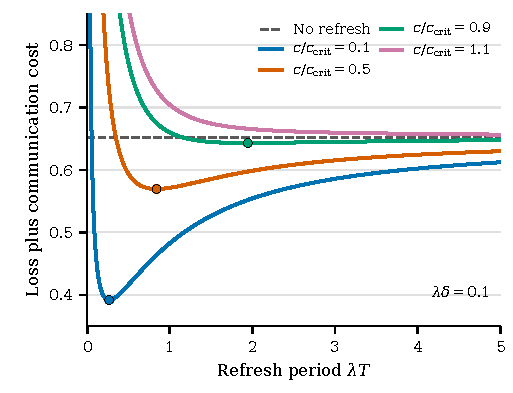
\includegraphics[width=\columnwidth]{figures/refresh_cost.pdf}
 \caption{Average team loss plus communication cost with periodic refreshing. Below the critical communication cost, each curve has a unique finite minimizer. Above it, fresh-local operation attains the minimum average cost.}
 \label{fig:refresh}
\end{figure}

To illustrate unequal rates, add an independent component with $a_2=0.4$, $b_2=0.8$, and $\lambda_2=0.12$, keeping $n=8$, $\kappa_2=1$, and unit weights for both components. At latency $0.1$, the slow component supplies $34.2\%$ of the value at reception and $81.2\%$ of the integrated gain $c_{\rm crit}$. The joint threshold is $1.1807$. At half this threshold, the optimal period is $5.5513$ and the total average cost is $0.9072$. Thus a component's contribution to the refresh decision depends on both the magnitude and the duration of its useful information.

\section{Conclusion}
Fresh local readings yield lower team loss than a complete delayed pool once its age exceeds an explicit threshold. Retaining fresh local observations preserves a positive pooling benefit at every finite age. This benefit decays at twice the signal's correlation decay rate, and its finite lifetime value determines when communication is worth its price and how often to refresh. The pooling law extends to unequal sensor quality and independent components with different rates. Different signal and sensor-error rates within a component, or observation-dependent refresh schedules, require further analysis.

Simulation code and extended analysis are available at \url{https://github.com/anrgusc/TINA}. Supplementary proof-review reports use Lamport-style hierarchies to record assumptions and logical dependencies.

\begin{samepage}
\section*{Acknowledgment}
OpenAI ChatGPT (Codex, \url{https://chatgpt.com}) was used to generate the abstract, text in Sections I--VII, and captions, and to assist with mathematical derivations and numerical code.
\end{samepage}

\begin{thebibliography}{13}
\bibitem{radner1962team} R. Radner, ``Team decision problems,'' \emph{Ann. Math. Statist.}, vol. 33, no. 3, pp. 857--881, 1962.
\bibitem{afshari2017static} M. Afshari and A. Mahajan, ``Static teams with common information,'' \emph{IFAC-PapersOnLine}, vol. 50, no. 1, pp. 11926--11931, 2017.
\bibitem{witsenhausen1971separation} H. S. Witsenhausen, ``Separation of estimation and control for discrete time systems,'' \emph{Proc. IEEE}, vol. 59, no. 11, pp. 1557--1566, Nov. 1971.
\bibitem{nayyar2011sharing} A. Nayyar, A. Mahajan, and D. Teneketzis, ``Optimal control strategies in delayed sharing information structures,'' \emph{IEEE Trans. Autom. Control}, vol. 56, no. 7, pp. 1606--1620, Jul. 2011.
\bibitem{yates2021aoi} R. D. Yates, Y. Sun, D. R. Brown, S. K. Kaul, E. Modiano, and S. Ulukus, ``Age of information: An introduction and survey,'' \emph{IEEE J. Sel. Areas Commun.}, vol. 39, no. 5, pp. 1183--1210, 2021.
\bibitem{sun2017update} Y. Sun, E. Uysal-Biyikoglu, R. D. Yates, C. E. Koksal, and N. B. Shroff, ``Update or wait: How to keep your data fresh,'' \emph{IEEE Trans. Inf. Theory}, vol. 63, no. 11, pp. 7492--7508, 2017.
\bibitem{ornee2021ou} T. Z. Ornee and Y. Sun, ``Sampling and remote estimation for the Ornstein--Uhlenbeck process through queues: Age of information and beyond,'' \emph{IEEE/ACM Trans. Netw.}, vol. 29, no. 5, pp. 1962--1975, 2021.
\bibitem{ballotta2023latency} L. Ballotta, M. R. Jovanovi{\'c}, and L. Schenato, ``Can decentralized control outperform centralized? The role of communication latency,'' \emph{IEEE Trans. Control Netw. Syst.}, vol. 10, no. 3, pp. 1629--1640, 2023.
\bibitem{ballotta2026role} L. Ballotta, J. Arbelaiz, V. Gupta, L. Schenato, and M. R. Jovanovi{\'c}, ``The role of communication delays in the optimal control of spatially invariant systems,'' \emph{IEEE Trans. Autom. Control}, vol. 71, no. 2, pp. 978--993, Feb. 2026, doi: \href{https://doi.org/10.1109/TAC.2025.3601758}{10.1109/TAC.2025.3601758}.
\bibitem{kar2012controlled} S. Kar and P. K. Varshney, ``Controlled collaboration for linear coherent estimation in wireless sensor networks,'' in \emph{Proc. 50th Annu. Allerton Conf. Commun., Control, Comput.}, 2012, pp. 334--341.
\bibitem{nayyar2013optimal} A. Nayyar, T. Ba\c{s}ar, D. Teneketzis, and V. V. Veeravalli, ``Optimal strategies for communication and remote estimation with an energy harvesting sensor,'' \emph{IEEE Trans. Autom. Control}, vol. 58, no. 9, pp. 2246--2260, Sep. 2013.
\bibitem{tina2026} S. Moeller and B. Krishnamachari, ``A theory of information architecture for networked decisions: Freshness, locality, and coordination,'' arXiv:2609.06351v1, 2026.
\bibitem{uhlenbeck1930brownian} G. E. Uhlenbeck and L. S. Ornstein, ``On the theory of the Brownian motion,'' \emph{Phys. Rev.}, vol. 36, no. 5, pp. 823--841, 1930, doi: \href{https://doi.org/10.1103/PhysRev.36.823}{10.1103/PhysRev.36.823}.
\end{thebibliography}
\end{document}
